\chapter{Theory of Debt, Its Proper Role, and Leverage Cycles}

This chapter follows Robert J. Shiller's eighth lecture in Yale's Financial Markets course, curated for the LazyingArt LLC track. The lecture begins with a puzzle that is older than modern finance: why are interest rates usually positive at all, and why are they so often only a few percent per year? Shiller answers that puzzle in stages. He begins with Bohm-Bawerk's verbal explanations, moves to Irving Fisher's two-period geometry, turns from geometry to the arithmetic of bond pricing and present value, and then returns to the institutional and moral question that had been deferred: if lending can raise welfare, why has interest so often been condemned? The sequence matters. The mathematics is not self-justifying; it is preparation for a judgment about what debt markets are doing in real social life.

\section{Why interest rates need an explanation}

An interest rate is the percentage one earns on a loan or pays on a loan. That sounds elementary, but the lecture asks us not to slide past the mystery. Interest rates have existed for thousands of years. They are often positive, and they are often not absurdly large. Why should the number be positive? Why not zero? Why not negative? Why should it so often lie in the neighborhood of a few percent rather than some utterly different scale?

Shiller begins historically because older thought framed the problem before modern diagrams did. In Bohm-Bawerk's late nineteenth-century theory of interest, three broad causes are offered.

\begin{itemize}
\item Technical progress: future production may be higher because knowledge improves over time.
\item Roundaboutness: production that takes time, including tool-making and indirect methods, may be more productive than immediate production.
\item Time preference: people may prefer present consumption to future consumption, so impatience itself enters the determination of interest.
\end{itemize}

The lecture emphasizes that this is not yet mathematical economics. It is literary economics: rich, suggestive, and historically important, but not yet organized into a single equilibrium picture. Fisher's contribution is to take these verbal causes and place them inside a disciplined two-period model.

\section{From Bohm-Bawerk to Fisher's two-period framework}

The textbook distillation of Fisher, as Shiller presents it, is a supply-and-demand diagram for saving. On one axis lies the quantity of saving; on the other lies the interest rate. Higher rates elicit more saving, so supply slopes upward. Lower rates stimulate more demand for investment funds, so demand slopes downward. Their intersection gives an equilibrium interest rate. This is useful, but Shiller deliberately leaves it behind because it compresses too much of the story.

Fisher's richer diagram uses two periods. On the horizontal axis we place current consumption, and on the vertical axis we place consumption next year. The lecture turns to a Robinson Crusoe economy because one person on an island is enough to show where the intertemporal tradeoff comes from.

Suppose Crusoe begins with a grain endowment \(e\). If he consumes \(c_0\) today, then \(e-c_0\) is the amount saved and planted. In a cleaned notation consistent with the lecture's story, the linear technology case may be written as
\begin{equation}
c_1=(1+r)(e-c_0),
\end{equation}
where \(c_1\) is next year's consumption and \(r\) is the interest rate implicit in the technology. The production possibility frontier is then a straight line with slope
\begin{equation}
\frac{dc_1}{dc_0}=-(1+r).
\end{equation}

The lecture's concrete illustration is that one bushel planted this year may yield two bushels next year. In that stripped-down case, \(1+r=2\). The frontier is linear, and technology alone fixes the slope. At this stage, roundaboutness is visible, and technical progress may also be folded in, but impatience is not yet doing the real work.

\begin{figure}[t]
\centering

\includegraphics[width=0.82\textwidth]{lecture_08_figure_02.png}
\caption{Irving Fisher board and cropped two-period graph. The board establishes the historical framing; the transcript supplies the economic content of the diagram.}
\end{figure}

Once diminishing returns are admitted, the picture becomes more interesting. Planting a little grain may be highly productive, while planting more and more grain pushes Crusoe onto worse land or weaker methods, so the extra future output from additional saving declines. The production possibility frontier bends inward, and the equilibrium is no longer pinned down by technology alone.

\begin{figure}[t]
\centering
\begin{tikzpicture}[scale=1.0]
\draw[->] (0,0) -- (6.2,0) node[below] {$c_0$};
\draw[->] (0,0) -- (0,5.2) node[left] {$c_1$};
\draw[thick] (0.4,4.7) .. controls (1.3,4.5) and (3.4,3.1) .. (5.3,0.4);
\draw[dashed] (0.7,4.3) -- (5.8,1.0);
\draw[thick] (0.6,4.1) .. controls (1.8,3.8) and (3.3,2.7) .. (5.0,1.5);
\fill (5.3,0.4) circle (1.5pt) node[below right] {$e$};
\fill (2.95,2.85) circle (1.5pt) node[above right] {$P^\ast$};
\node at (4.8,4.25) {PPF};
\node at (4.8,2.25) {$u^\ast$};
\node at (4.15,0.8) {$-(1+r)$};
\end{tikzpicture}
\caption{Cleaned reconstruction of Fisher's one-person two-period geometry. The transcript, rather than the cropped image alone, supports the labels and economic interpretation.}
\end{figure}

The crucial point is that a theory of interest must explain more than a supply-demand crossing. It must explain the slope of an intertemporal opportunity set and its interaction with preferences.

\section{Robinson Crusoe, first alone and then in a lending market}

With diminishing returns, Crusoe chooses the highest indifference curve tangent to the production possibility frontier. At the tangency, the marginal rate at which he is willing to trade off present for future consumption equals the marginal rate allowed by production:
\begin{equation}
\mathrm{MRS}_{c_0,c_1}=\mathrm{MRT}_{c_0,c_1}=1+r.
\end{equation}

Now Bohm-Bawerk's three causes coexist in one picture. The frontier carries roundaboutness and productivity. Technical progress can shift the frontier itself. Time preference appears in the shape and slope of the indifference curves. The interest rate is therefore not just impatience and not just technology. It is the slope at a tangency between opportunities and preferences.

This also gives an immediate comparative statics result. If Crusoe becomes more impatient, his indifference curves tilt so as to favor present consumption more strongly. The tangency moves to the right: more consumption now, less later, and a steeper frontier at the chosen point. In the language of the lecture, greater impatience raises the interest rate.

Shiller then adds a second Crusoe. They have the same technology and the same endowment, but not the same patience. One wants to consume more today; the other is willing to defer more toward next year. If they remain isolated on opposite sides of the island, each chooses a separate tangency on the same production possibility frontier. But the moment they discover each other, the possibility of a loan appears.

The key observation is not just that tastes differ. It is that marginal productivity differs at their separate production plans. The patient Crusoe is planting so much that diminishing returns have set in hard. The impatient Crusoe is planting so little that marginal productivity is still high. A loan reallocates grain toward the more productive margin while also allowing each person to move toward a preferred consumption profile.

\begin{figure}[t]
\centering
\begin{tikzpicture}[scale=1.0]
\draw[->] (0,0) -- (6.2,0) node[below] {$c_0$};
\draw[->] (0,0) -- (0,5.2) node[left] {$c_1$};
\draw[thick] (0.4,4.7) .. controls (1.4,4.45) and (3.5,3.15) .. (5.35,0.4);
\draw[dashed] (0.6,4.35) -- (5.85,0.95);
\fill (3.0,2.8) circle (1.5pt) node[above right] {$P$};
\fill (4.45,1.86) circle (1.5pt) node[right] {$A$};
\fill (1.85,3.54) circle (1.5pt) node[left] {$B$};
\draw[thick] (3.0,3.15) .. controls (3.45,2.85) and (3.95,2.3) .. (5.15,1.66);
\draw[thick] (0.95,3.95) .. controls (1.25,3.9) and (1.55,3.72) .. (2.75,3.0);
\node at (4.9,4.25) {PPF};
\node at (4.9,2.55) {$u_A$};
\node at (1.2,3.2) {$u_B$};
\end{tikzpicture}
\caption{Two Crusoes with different patience. Production occurs at the common tangent point \(P\), while the lending market supports different consumption points \(A\) and \(B\) on the same intertemporal budget line.}
\end{figure}

The market rate is the slope of the common tangent line. That is the lecture's core theoretical claim. The interest rate is not read off from one person's character. It emerges from technology, diminishing returns, and heterogeneous preferences together.

\subsection{Question \& Answer}

\paragraph{Question.} Why is a loan socially useful in the Fisher story?

\paragraph{Answer.} Because the two agents are not merely different; they are located at different marginal productivities. The impatient Crusoe wants present consumption and is planting too little from the standpoint of future productivity. The patient Crusoe is willing to defer consumption but is planting so much that extra saving earns little. A loan lets one consume more now and the other plant where returns are higher. The common tangent line represents exactly this mutually beneficial reallocation. In the model, both agents reach higher utility than under isolation.

That is why the lecture pauses here and says, in effect: the lending market now looks plainly good. Shiller does not reject that conclusion. He postpones the criticism of lending until the end, after the arithmetic has been laid out.

\section{Debt arithmetic: discount bonds, compounding, and present discounted value}

At this point the lecture changes level. We are asked to take the Fisher story as a theory of interest and then move into the arithmetic of finance. The first instrument is the simplest one: the discount bond.

A discount bond pays a fixed amount at maturity and no coupon along the way. If the face value is \(100\) at date \(T\), then under annual compounding the current price is
\begin{align}
p &= \frac{100}{(1+r)^T}, \\
(1+r)^T &= \frac{100}{p}, \\
r &= \left(\frac{100}{p}\right)^{1/T}-1.
\end{align}
The rate \(r\) inferred from the price is the yield to maturity.

\paragraph{Worked example.} If the bond matures in two years, then
\begin{equation}
p=\frac{100}{(1+r)^2}
\qquad\Longrightarrow\qquad
r=\sqrt{\frac{100}{p}}-1.
\end{equation}
This is the simplest form of the lecture's message: a bond quote can be translated into an annual interest rate once the compounding convention is fixed.

Shiller then slows down over compounding. Under annual compounding, interest on interest begins only after a full year. But many financial conventions are semiannual, not annual, because many bonds pay coupons every six months. To keep the notation stable, it is best to normalize the lecture as follows:
\begin{equation}
z=\frac{r}{2}, \qquad n=2T, \qquad p=\frac{100}{(1+z)^n}.
\end{equation}
Here \(z\) is the half-year rate and \(n\) counts half-year periods.

\begin{figure}[t]
\centering

\includegraphics[width=0.82\textwidth]{lecture_08_figure_03.png}
\caption{Annual versus continuous compounding on the board. The visible exponential term anchors the passage to the limit case of continuous compounding.}
\end{figure}

The lecture then takes the limit of more and more frequent compounding. In cleaned notation,
\begin{equation}
B(T)=B_0\lim_{m\to\infty}\left(1+\frac{r}{m}\right)^{mT}=B_0 e^{rT}.
\end{equation}
This is the continuous-compounding balance formula written on the board in partial form. It says that the balance after time \(T\) is the initial amount times \(e^{rT}\).

\begin{definition}
The present discounted value, or \(\mathrm{PDV}\), of a payment stream is the amount today that is financially equivalent to that stream once the relevant interest-rate convention has been specified.
\end{definition}

For a single payment \(x\) at date \(T\), the annual-compounding formula is
\begin{equation}
\mathrm{PDV}=\frac{x}{(1+r)^T}.
\end{equation}
For a sequence of annual payments \(\{x_t\}\),
\begin{equation}
\mathrm{PDV}=\sum_{t=1}^{\infty}\frac{x_t}{(1+r)^t}.
\end{equation}
For semiannual payments one writes, with the lecture's convention,
\begin{equation}
\mathrm{PDV}=\sum_{t=1}^{\infty}\frac{x_t}{(1+r/2)^t}.
\end{equation}
And for a continuously paid stream \(x(t)\),
\begin{equation}
\mathrm{PDV}=\int_0^\infty x(t)e^{-rt}\,dt.
\end{equation}

This is why present discounted value is the central technical concept of the lecture. Once a future stream has been collapsed into a present number, many different debt contracts can be compared within one common language.

\section{Perpetuities, annuities, and conventional bonds}

Shiller next specializes \(\mathrm{PDV}\) into the named payment streams that appear again and again in finance. The order matters: consol first, annuity second, conventional bond third.

\begin{figure}[t]
\centering

\includegraphics[width=0.82\textwidth]{lecture_08_figure_04.png}
\caption{Annuity setup beside the consol benchmark. The board preserves the live transition from perpetuity language to a finite payment stream.}
\end{figure}

A consol, or perpetuity, pays the same coupon forever. On the board Shiller writes the special case of a British consol paying one pound per year:
\begin{equation}
\mathrm{PDV}_{\text{consol}}=\frac{\pounds 1}{r}.
\end{equation}
In normalized form,
\begin{equation}
\mathrm{PDV}_{\text{consol}}=\frac{C}{r},
\qquad
r=\frac{C}{\mathrm{PDV}_{\text{consol}}}.
\end{equation}
The formula is simple because the bond never matures. Price is coupon divided by interest rate.

An annuity is the finite version: a fixed payment \(x\) each period from \(t=1\) through \(t=T\), and then nothing. The lecture writes the annuity formula directly, but its structure is especially clear if we derive it from the perpetuity. An annuity is a perpetuity minus the tail that begins after date \(T\):
\begin{align}
\mathrm{PDV}_{\text{annuity}}
&= \frac{x}{r}-\frac{x}{r(1+r)^T} \\
&= \frac{x}{r}\left(1-\frac{1}{(1+r)^T}\right).
\end{align}
That is exactly the board formula.

\begin{figure}[t]
\centering

\includegraphics[width=0.82\textwidth]{lecture_08_figure_05.png}
\caption{Finite-annuity formula applied to a conventional bond. The board links the annuity calculation directly to bond coupons.}
\end{figure}

This matters because many actual contracts are annuities in disguise. The lecture gives the familiar example of a traditional home mortgage: fixed periodic payments for a long but finite horizon.

A conventional bond is one step more complicated. It pays coupon \(C\) every six months and then repays principal at maturity. The board states the decomposition more clearly than the full algebra, so it is best to write the cleaned formula explicitly:
\begin{equation}
\mathrm{PDV}_{\text{bond}}=
\frac{C}{z}\left(1-\frac{1}{(1+z)^n}\right)+\frac{F}{(1+z)^n},
\qquad
z=\frac{r}{2}, \quad n=2T.
\end{equation}
The first term is the coupon annuity. The second is the discounted principal. The final coupon is already included in the annuity term, while the separate principal repayment is the discount-bond term.

\begin{figure}[t]
\centering
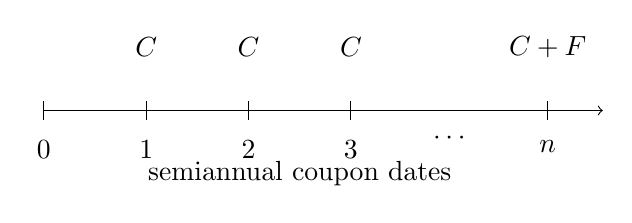
\begin{tikzpicture}[scale=1.0]
\draw[->] (0,0) -- (7.1,0);
\draw (0,0.12) -- (0,-0.12) node[below=4pt] {$0$};
\draw (1.3,0.12) -- (1.3,-0.12) node[below=4pt] {$1$};
\draw (2.6,0.12) -- (2.6,-0.12) node[below=4pt] {$2$};
\draw (3.9,0.12) -- (3.9,-0.12) node[below=4pt] {$3$};
\draw (6.4,0.12) -- (6.4,-0.12) node[below=4pt] {$n$};
\node at (1.3,0.8) {$C$};
\node at (2.6,0.8) {$C$};
\node at (3.9,0.8) {$C$};
\node at (5.15,-0.35) {$\cdots$};
\node at (6.4,0.8) {$C+F$};
\node at (3.25,-0.8) {semiannual coupon dates};
\end{tikzpicture}
\caption{Coupon timeline for a conventional bond. The cash-flow structure is exactly what the annuity-plus-principal decomposition captures.}
\end{figure}

\section{Forward rates from the term structure}

The lecture's next move is motivated by Sir John Hicks. The term structure of interest rates is a list of yields, today, for many maturities: one year, two years, ten years, thirty years, and so on. But Hicks's insight was that from these rates quoted today we can also infer rates between two future dates.

Shiller frames the question as a coffee-hour puzzle in 1925. Open the paper and read the rates quoted from now to various future dates. But what if we want the one-year rate from 1926 to 1927, as inferred already in 1925? That is the forward rate.

\begin{figure}[t]
\centering

\includegraphics[width=0.82\textwidth]{lecture_08_figure_06.png}
\caption{Forward-rate identity and expectations-theory trading setup. The board combines the algebra with the 1925--1926 trade construction.}
\end{figure}

\subsection{Question \& Answer}

\paragraph{Question.} How can we lock in a one-year interest rate for a future year using only bonds traded today?

\paragraph{Answer.} Let \(r_1\) be today's one-year yield and \(r_2\) today's two-year yield. Suppose we expect to have \(\pounds 100\) to invest in 1926 and want to lock in, already in 1925, the return from 1926 to 1927. The lecture's strategy is to buy
\[
\frac{(1+r_2)^2}{1+r_1}
\]
two-year discount bonds in 1925 and simultaneously short one one-period bond.

At date 1926, the short one-period bond creates an obligation of \(\pounds 100\). By construction, that is the amount we were planning to invest in 1926. At date 1927, the long position pays
\[
\pounds 100\cdot \frac{(1+r_2)^2}{1+r_1}.
\]
Therefore the gross return from 1926 to 1927 is
\begin{align}
1+f &= \frac{(1+r_2)^2}{1+r_1}, \\
f &= \frac{(1+r_2)^2}{1+r_1}-1.
\end{align}

\begin{figure}[t]
\centering
\begin{tikzpicture}[scale=1.0]
\draw[->] (0,0) -- (6.8,0);
\draw (0,0.12) -- (0,-0.12) node[below=4pt] {$1925$};
\draw (3,0.12) -- (3,-0.12) node[below=4pt] {$1926$};
\draw (6,0.12) -- (6,-0.12) node[below=4pt] {$1927$};
\node[align=center] at (0,0.95) {long $\dfrac{(1+r_2)^2}{1+r_1}$\\ two-year bonds};
\node[align=center] at (0,-1.0) {short $1$\\ one-period bond};
\draw[->] (3,0) -- (3,-0.8);
\node at (3,-1.15) {$-\pounds 100$};
\draw[->] (6,0) -- (6,1.0);
\node at (6,1.4) {$+\pounds 100\,\dfrac{(1+r_2)^2}{1+r_1}$};
\end{tikzpicture}
\caption{Timeline for the one-step forward-rate construction. The trade locks in the gross return between 1926 and 1927 using positions chosen in 1925.}
\end{figure}

This is the lecture's most important term-structure identity in worked form. The market already contains, implicitly, rates between future dates.

The expectations theory then gives this identity an interpretation. In compact notation one writes
\begin{equation}
f \approx \mathbb{E}_t\!\left[r^{\text{spot}}_{t+1}\right].
\end{equation}
That is, the forward rate quoted today is interpreted as the expected future spot rate.

But Hicks's own qualification, stressed by Shiller, is that this cannot be the whole story. Forward rates tend to lie above the optimally forecast future spot rate because investors demand compensation for bearing risk. In a compact cleaned notation,
\begin{equation}
f=\mathbb{E}_t\!\left[r^{\text{spot}}_{t+1}\right]+\pi,
\qquad
\pi>0.
\end{equation}
So the term structure is not just a map of expectations. It also contains risk premia.

\section{From the theory of interest to the problem of usury}

Only after the technical material is in place does the lecture return to the question it deliberately postponed. The Fisher story makes lending look clean and socially useful. Two people with different intertemporal preferences discover each other, form a loan, and both become better off. Why, then, has interest so often been treated as morally suspect?

Shiller answers by stepping back into history. The old language of usury is important precisely because it is ambiguous. The Latin \emph{usura} can mean interest, but it can also mean excessive or abusive interest. Similar ambiguities surround the religious condemnations in older Christian and Islamic traditions. The lecture does not try to settle the philology. Instead it asks why suspicion of lending persisted for so long if the Fisher logic is basically right.

\subsection{Question \& Answer}

\paragraph{Question.} If lending raises welfare in the Fisher story, why has interest so often been condemned?

\paragraph{Answer.} Because in real debt markets differences in intertemporal choice are not always harmless differences in taste. They may reflect error, impulsiveness, ignorance, distress, or manipulation. In the Crusoe model, one person's desire for present consumption is simply a preference. In real life, it may be a mistake that ought to be corrected by advice rather than amplified by a loan. That is where usury enters: not as any interest payment whatsoever, but as lending undertaken without genuine concern for the borrower's welfare.

This is why the lecture turns to behavioral economics. A lender can do something socially useful by helping a household smooth consumption or finance a genuinely productive project. But a lender can also prey on short-run temptation, poor information, or desperation. Shiller's examples are deliberately provocative: vacation loans, honeymoon loans, and the advertising machinery that normalizes borrowing for impulses that may or may not be wise. The point is not that every such loan is wrong. Indeed, the lecture preserves Modigliani's suggestion that some expenditures, including a honeymoon, may plausibly be viewed as investments in a life and a relationship. The point is that one cannot tell the whole moral story from the Fisher diagram alone.

The same theme appears in the closing discussion of Elizabeth Warren. Her work on bankruptcy and household distress is introduced to show that credit markets can systematically exploit people, and that financial innovation is not always aligned with borrower welfare. The institutional response, in Shiller's telling, is not to repudiate debt markets. It is to regulate them. The Consumer Financial Protection Bureau appears in the lecture as a modern expression of an old concern: if debt markets are useful, they must still be guarded against abuse.

So the lecture's conclusion is deliberately balanced. The original Fisher and Bohm-Bawerk story about interest is not discarded. It is affirmed. Even loans for apparently soft purposes are not automatically illegitimate. But the older suspicion of usury is not nonsense either. It survives because real lending can become behaviorally exploitative, and because good debt markets require government rules that prevent abuse.

\section{Summary}

The lecture begins with a mystery about why interest exists and ends with a judgment about when lending is socially acceptable. Between those endpoints, it develops a coherent chain. Bohm-Bawerk names the causes of interest. Fisher turns them into a two-period geometry in which the interest rate is the slope of a common tangent shaped jointly by productivity and preferences. The arithmetic of finance then converts future payments into present values through discounting, compounding, perpetuities, annuities, and conventional bonds. Finally, the term structure yields forward rates, and forward rates lead to the question of what markets are forecasting and what premia they contain. None of this settles the moral question by itself. Shiller's final position is that debt is useful, often essential, and theoretically well-grounded, but still in need of regulation because useful lending and usury are not the same thing.